\documentclass[a4paper,oneside,titlepage]{article}

% language settings
\usepackage[english]{babel}
\usepackage[utf8]{inputenc}
\usepackage[T1]{fontenc}

% includes
\usepackage{float}
\usepackage{pdfpages}
\usepackage{color}
\usepackage{wrapfig}
\usepackage{graphicx}
\usepackage{caption}
\usepackage{subcaption}
\usepackage{hyperref}
\usepackage{fancyhdr}

% document information
\title{MassIdea \\ Meeting Minutes: Matchmaking}
\author{Jan Michael Auer \and Martin Hanner \and Lisa Jedinger}
\date{June 11, 2012}

% header and footer definition
\setlength{\headheight}{15.2pt}
\pagestyle{fancy}
\lhead{Meeting Protocol: Matchmaking}\rhead{June 11, 2012}
\cfoot{\thepage}

% overrides
\setlength{\parindent}{0pt}
\setlength{\parskip}{.66\baselineskip}

\begin{document}
\maketitle
	
\tableofcontents
\vspace{5\baselineskip}	
\section{Agenda}
	
The project meeting was scheduled for two days, 4 hours each. 

\begin{description}
	\item[Monday] On the first day, a discussion about the current status was planned. This includes a presentation of the last semester and review of the running system including the new layout.
	\item[Tuesday] Tuesday was reserved for future orientation. After a short presentation of the milestone plan for the coming semester, there were over three hours scheduled for creativity and generating ideas.
\end{description}

\pagebreak

\section{Monday}

\subsection{Participants}

\begin{description}
	\item[Customer] Teemu Santonen
	\item[Coaches] Josef Altmann
	\item[Team] Jan Michael Auer, Martin Chalupar, Tobias Curth, Martin Hanner, Lisa Jedinger, Michael Lang, Florian Paar, Jürgen Wimmer
\end{description}

\subsection{Description}

The meeting started with a presentation of results of the last semester and the current state of the implementation. This included a brief overview of the past milestones and achieved results.
In great detail, we presented the new layout of the start page with the new logo of Massidea. The customer appreciated the new layout and was pleased about its implementation in the Zend system. In the feedback session the customer decided to change the colors of the three big sections to brighter ones.

The remaining time was used to discuss the product backlog, which the customer had received a week before. A final prioritization for the first items in the list was achieved. While discussing the other items, the team started a brainstorming session about a match-making functionality. This functionality in combination with the new projects should determine the innovative part of Massidea.

\subsection{Results}

\begin{itemize}
	\item As requested by the customer, the colors of the three big sections (\emph{Challenges}, \emph{Visions} and \emph{Ideas}) and subsequently also those in the logo were changed.
	\item The prioritized Backlog
	\item Projects need additional structure to be useful for potential users. Therefore, project administrators will be able to create tasks which they can assign users to. Such tasks should be matched with similar tasks of other projects, which might lead to collaboration of two or more project teams. Elaboration of details was subject of the next day.
\end{itemize}

% eventuell grafiken ergänzen

\pagebreak
\section{Tuesday}

\subsection{Participants}

\begin{description}
	\item[Customer] Teemu Santonen
	\item[Coaches] Josef Altmann, Martina Gaisch
	\item[Team] Jan Michael Auer, Martin Chalupar, Tobias Curth, Martin Hanner, Lisa Jedinger, Michael Lang, Florian Paar, Sabrina Schwarzgruber, Jürgen Wimmer
\end{description}

\subsection{Description}

Tobias started the meeting by presenting the changes of the start page. After that, the milestone plan for the winter semester was presented by Sabrina.
The main part of the meeting was to generate ideas for the match-making tool.
First, a persona was defined to get a feeling how the system will be used.
The team set up three task forces, each of which had to present its results. After the presentations the pros and cons of the results were discussed with the customer. In general, there existed two iterations and the task forces had to adapt their results from the first iteration during the second iteration. In the last step --- the third iteration --- the task forces were rearranged, in order to transfer the ideas into one system. Afterwards the ideas were discussed with the user, Martina Gaisch, and the customer, who gave us useful feedback. 

\subsection{Results}

\emph{Note:} For reasons of clarity and comprehensibility, all illustrations and graphics are placed in the \emph{Appendix} on Page~\pageref{sec:appendix} ff.

\subsubsection[Personas]{Persona: Martina Gaisch}

\begin{wrapfigure}{r}{0.25\textwidth}
	\vspace{-20pt}
  	\begin{center}
    
\includegraphics[width=0.2\textwidth]{gaisch}
  \end{center}
\end{wrapfigure}

Job: Teacher\\
Age group: 30-50

Martina Gaisch is an English teacher at the University of Applied Sciences Upper Austria. A main part of her work is intercultural communication. She has average computer skills and searches for a platform, where she is able to establish international contacts. She wants to find other teachers for corporate projects. In addition to this, she is interested in sharing documents over the platform.

\subsubsection{Usecases}

The usecase diagram (see Figure~\ref{usecase}) shows the identified features from the idea generating process concerning match-making.

\subsubsection{Capabilities and Workflow}

The project administrator is able to choose one of his projects from the right menu. The ``manage projects'' page allows to choose from several contents by selecting a menu entry on the left. The interactive sidebar fits to the content accordingly. The user is able to switch the content by choosing a page from the left menu. (Figure~\ref{wireframe-manageproject}) 

Users can also create projects as specified in the System Requirements Specification. First of all, users have to create the project itself by supplying data like project name, short description, \dots 
The next step is to invite people to the project (Figure~\ref{wireframe-InvitePerson}). On the left side users can see the team members, who have already been added to the project and on the right side, there are suggestions given by the system of who might be suitable for the project.
This step is optional at this particular point, as it can be repeated at any time.

The next step is to add tasks to the project (Figure~\ref{wireframe-PlanTasks}). On the right side you can see a time line of the existing tasks. 
If there is at least one match for the task, it will be marked. 
In addition new tasks are created by filling in the displayed fields like task-name, description,...

Additionally, users are able to search for projects (Figure~\ref{search}) by simply entering keywords into the search field.
If users are not satisfied with the provided search results, they can use an extended search, where they can specify the search in greater detail. 
The results of the search will be displayed with two possible actions for each item: Read more or connect (invite people, merge tasks, \dots).
Users also have the possibility of creating a new insertion in the marketplace in order to attract attention.


\subsubsection{Insights}

\begin{description}
	\item[Omnipresent interactive sidebar] An interactive sidebar is a useful feature in the whole system. The sidebar displays generated related content based on the displayed page. For example, if the user is on the members page the sidebar shows people the user might know.
	\item[Marketplace] The marketplace is a feature which helps users to find resources like projects, members or other content. As marketplaces are known to almost every user of the internet, this is a very intuitive approach to offer and find services. 
\end{description}

\pagebreak
\section*{Appendix}
\label{sec:appendix}

\begin{figure}[h]
  	\centering
    \includegraphics[width=\textwidth]{"UseCase Workshop"}
  \caption{Usecase-diagramm}
  \label{usecase}
\end{figure}

\begin{figure}[h]
    \includegraphics[width=\textwidth]{"Wireframe ManageProject"}
  \caption{ManageProject}
  \label{wireframe-manageproject}
\end{figure}

\begin{figure}[h]
    \includegraphics[width=\textwidth]{"Wireframe InvitePerson"}
  \caption{InvitePerson}
  \label{wireframe-InvitePerson}
\end{figure}

\begin{figure}[h]
    \includegraphics[width=\textwidth]{"Wireframe PlanTasks"}
  \caption{PlanTasks}
  \label{wireframe-PlanTasks}
\end{figure}

\begin{figure}[h]
    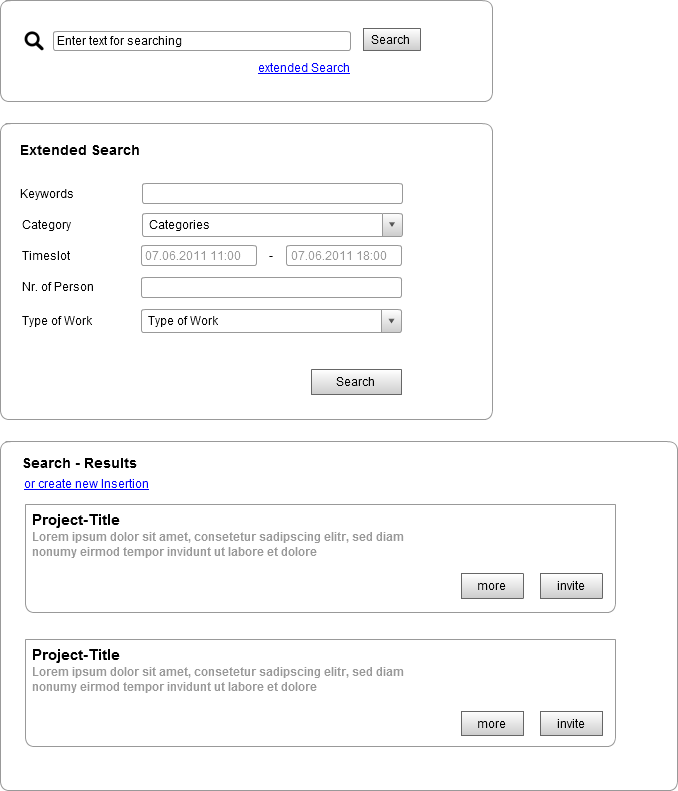
\includegraphics[width=\textwidth]{search}
  \caption{Search function}
  \label{search}
\end{figure}

\end{document}